\documentclass[9pt,twocolumn,twoside]{pnas-new}
% Use the lineno option to display guide line numbers if required.
% Note that the use of elements such as single-column equations
% may affect the guide line number alignment. 

\templatetype{pnasresearcharticle} % Choose template 
% {pnasresearcharticle} = Template for a two-column research article
% {pnasmathematics} = Template for a one-column mathematics article
% {pnasinvited} = Template for a PNAS invited submission

\newcommand*{\lpath}{./}%
%\usepackage[cmex10]{amsmath, mathtools}
\usepackage{amsmath,amssymb,amsbsy,amsfonts,amsthm}
\usepackage{mathtools}
\usepackage{multirow}
\usepackage{bm}
\usepackage{enumerate}
\usepackage{url}
%\usepackage[ruled,vlined]{algorithm2e}
\usepackage{fancyvrb}
\usepackage{yfonts}
\usepackage{wrapfig}
\usepackage{subfigure}
\usepackage{tikz}
\usetikzlibrary{bayesnet}
\newcommand{\tikzmark}[1]{\tikz[overlay,remember picture] \node (#1) {};}
\usepackage{calc}%    For the \widthof macro
\usepackage{xparse}%  For \NewDocumentCommand


%% Variable de compilation
\newif\ifbeamer
\beamerfalse
\newcommand{\beamer}[2]{\ifbeamer #1 \else #2 \fi}
%%%

%\usepackage[latin1]{inputenc}
\usepackage[utf8]{inputenc} % manage utf8 encodage 
%\usepackage[english]{babel} % for french document ! dirty enumerate style,+ bad change rectangle colors for section linking.
\usepackage{fancyhdr} % for heading
\usepackage{listings}
\usepackage[colorlinks=true, urlcolor=blue]{hyperref} % url, link
\usepackage{graphicx}
\usepackage{geometry}

%\usepackage[cmex10]{amsmath, mathtools}
\usepackage{amsmath,amssymb,amsbsy,amsfonts,amsthm}
\usepackage{multirow}
\usepackage{bm}
\usepackage{enumerate}
\usepackage{url}
\usepackage[ruled,vlined]{algorithm2e}
\usepackage{fancyvrb}
\usepackage{yfonts}

\usepackage{wrapfig}
\usepackage{tikz}
    %\input{../tikz.conf}
    
\usetikzlibrary{bayesnet}
    
%%%%%%%%%%% Box 
\usepackage{calc}%    For the \widthof macro
\usepackage{xparse}%  For \NewDocumentCommand
\newcommand{\tikzmark}[1]{\tikz[overlay,remember picture] \node (#1) {};}

%%%%%%%%%% Math
\renewcommand{\text}{\textnormal}
\newcommand{\pr}{\mathbf{p}}
\newcommand{\E}{\mathbb{E}}
\newcommand{\divkk}{\mathbb{K}}
\newcommand{\entropy}{\mathbb{H}}
\newcommand{\gem}{\mathrm{GEM}}
\newcommand{\Mult}{\mathrm{Mult}}
\newcommand{\DP}{\mathrm{DP}}
\newcommand{\IBP}{\mathrm{IBP}}
\newcommand{\M}{\mathcal{M}}
\newcommand{\V}{\mathcal{V}}
\newcommand{\N}{\mathcal{N}}
    
\makeatletter
\NewDocumentCommand{\DrawBox}{s O{}}{%
    \tikz[overlay,remember picture]{
    	\IfBooleanTF{#1}{%
    		\coordinate (RightPoint) at ($(left |- right)+(\linewidth-\labelsep-\labelwidth,0.0)$);
    	}{%
    	\coordinate (RightPoint) at (right.east);
    }%
    \draw[red,#2]
    ($(left)+(-0.2em,0.9em)$) rectangle
    ($(RightPoint)+(0.2em,-0.3em)$);}
}

\NewDocumentCommand{\DrawBoxWide}{s O{}}{%
	\tikz[overlay,remember picture]{
		\IfBooleanTF{#1}{%
			\coordinate (RightPoint) at ($(left |- right)+(\linewidth-\labelsep-\labelwidth,0.0)$);
		}{%
		\coordinate (RightPoint) at (right.east);
	}%
	\draw[red,#2]
	($(left)+(-\labelwidth,0.9em)$) rectangle
	($(RightPoint)+(0.2em,-0.3em)$);}
}
\makeatother
%%%%% ! Box

\geometry{
      a4paper,
	    body={160mm,260mm},
	    left=25mm,top=20mm,
	    headheight=4mm,headsep=8mm,
        footskip=10mm,
        }
                                              

%%%%%%%%%%%%%%%%%%%%%%%%%%%%%%%%%%%%%%%%%%%%%%%%%%%%%%%%%%%%%%%%%%%%%%%%%%%%%%%%%%%%%%%%%%%%%%%%%%%%%%
%%%%% => Internal
%%%%%%%%%%%%%%%%%%%%%%%%%%%%%%%%%%%%%%%%%%%%%%%%%%%%%%%%%%%%%%%%%%%%%%%%%%%%%%%%%%%%%%%%%%%%%%%%%%%%%%

% itemize item def
%% \begin{itemize}\itemsep2pt % example space betwew item
%\renewcommand{\FrenchLabelItem}{\textbullet}
\renewcommand{\labelitemi}{$\bullet$}
\renewcommand{\labelitemii}{$\cdot$}
\renewcommand{\labelitemiii}{$\diamond$}
\renewcommand{\labelitemiv}{$\ast$}

% equation reference
\renewcommand{\theequation}{\thesection.\arabic{equation}}

%%%%%%%%%%%%%%%%%%%%%%%%%%%%%%%%%%%%%%%%%%%%%%%%%%%%%%%%%%%%%%%%%%%%%%%%%%%%%%%%%%%%%%%%%%%%%%%%%%%%%%
%%%%% => Alias
%%%%%%%%%%%%%%%%%%%%%%%%%%%%%%%%%%%%%%%%%%%%%%%%%%%%%%%%%%%%%%%%%%%%%%%%%%%%%%%%%%%%%%%%%%%%%%%%%%%%%%

% write code
\lstnewenvironment{C}[1]
{\lstset{language=C,
      frame=tBRl,
      basicstyle=\scriptsize,stringstyle=\emph,showstringspaces=false,
      numbers=left,numberstyle=\tiny,
      breaklines=true, columns=flexible, title={#1}}
}{}
      
%%%%%%%%%%%%%%%%%%%%%%%%%%%%%%%%%%%%%%%%%%%%%%%%%%%%%%%%%%%%%%%%%%%%%%%%%%%%%%%%%%%%%%%%%%%%%%%%%%%%%%
%%%%% => Preambles Pages
%%%%%%%%%%%%%%%%%%%%%%%%%%%%%%%%%%%%%%%%%%%%%%%%%%%%%%%%%%%%%%%%%%%%%%%%%%%%%%%%%%%%%%%%%%%%%%%%%%%%%%

\pagestyle{fancy}
\fancyhf{} % remove default headers
\fancyfoot[C]{\thepage}
\renewcommand{\footrulewidth}{0.3pt}
\renewcommand{\headrulewidth}{0.3pt}

%%%%%%%%%% Math
\renewcommand{\text}{\textnormal}
\newcommand{\ifm}{\texttt{ILFM}}
\newcommand{\imb}{\texttt{IMMSB}}
\newcommand{\pr}{p}
\newcommand{\p}{p}
\newcommand{\E}{\mathbb{E}}
\newcommand{\divkk}{\mathbb{K}}
\newcommand{\entropy}{\mathbb{H}}
\newcommand{\gem}{\mathrm{GEM}}
\newcommand{\Mult}{\mathrm{Mult}}
\newcommand{\DP}{\mathrm{DP}}
\newcommand{\IBP}{\mathrm{IBP}}
\newcommand{\M}{\mathcal{M}}
\newcommand{\V}{\mathcal{V}}
\newcommand{\N}{\mathcal{N}}
\newcommand{\mat}[1]{\mathbf{#1}}
\newcommand{\unit}{1\!\!1}

\newtheorem{definition}{Definition}[section]
\newtheorem{proposition}{Proposition}[section]
\newtheorem{theorem}{Theorem}[section]
\newtheorem{corollary}{Corollary}[section]


\title{Stochastic mixed membership models and link prediction: a study of homophily and preferential attachment in social networks}

% Use letters for affiliations, numbers to show equal authorship (if applicable) and to indicate the corresponding author
\author[a,b]{Adrien Dulac}
\author[a]{Eric Gaussier} 
\author[b,1]{Christine Largeron}

\affil[a]{Univ. Grenoble Alpes, CNRS, Grenoble INP, LIG - F-38000 Grenoble}
\affil[b]{Universit\'e Jean Monnet, Laboratoire Hubert Curien - F-42000 Saint-Etienne}
%\affil[c]{Affiliation Three}

% Please give the surname of the lead author for the running footer
\leadauthor{Dulac} 

% Please add here a significance statement to explain the relevance of your work
\significancestatement{We introduce formal definitions of the compliance of probabilistic link prediction models to homophily and preferential attachment in social networks, and show that standard stochastic mixed membership models comply with homophily with the similarity that underlies them. For preferential attachment, the situation is more contrasted: if these models do not comply with global preferential attachement, their compliance to local preferential attachment depends on whether the memberships to latent factors are hard or soft.}

% Please include corresponding author, author contribution and author declaration information
\authorcontributions{All authors contributed equally to the theoretical development and experimental design. A. Dulac furthermore implemented all the models and ran the experiments.}
%\authordeclaration{Please declare any conflict of interest here.}
%\equalauthors{\textsuperscript{1}A. Dulac, E. Gaussier and C. Largeron contributed equally to this work.}
\correspondingauthor{\textsuperscript{1}To whom correspondence should be addressed. E-mail: Christine.Largeron@univ-st-etienne.fr}

% Keywords are not mandatory, but authors are strongly encouraged to provide them. If provided, please include two to five keywords, separated by the pipe symbol, e.g:
\keywords{Stochastic mixed membership models $|$ Social networks $|$ Homophily $|$ Preferential attachment} 

\begin{abstract}
We assess here whether standard stochastic mixed membership models are adapted to link prediction in social networks by studying how they handle homophily and preferential attachment. To do so, we introduce formal definitions of the compliance of probabilistic link prediction models to homophily and preferential attachment. Our theoretical analysis reveals that standard stochastic mixed membership models comply with homophily with the similarity that underlies them. For preferential attachment, the situation is more contrasted: if these models do not comply with global preferential attachement, their compliance to local preferential attachment depends on whether the memberships to latent factors are hard or soft. We illustrate these elements on synthetic and real networks.
\end{abstract}

\dates{This manuscript was compiled on \today}
\doi{\url{www.pnas.org/cgi/doi/10.1073/pnas.XXXXXXXXXX}}

\begin{document}

\verticaladjustment{-2pt}

\maketitle
\thispagestyle{firststyle}
\ifthenelse{\boolean{shortarticle}}{\ifthenelse{\boolean{singlecolumn}}{\abscontentformatted}{\abscontent}}{}

\label{sec:intro}

Several powerful relational learning models have been proposed to solve the problem commonly referred to as \textit{link prediction} that consists in predicting the likelihood of a future association between two nodes in a network \cite{Liben-Nowell07, HassanZaki11}. Among such models, the class of stochastic mixed membership models has received much attention as such models can be used to discover hidden properties and infer new links in social networks. Two main models in this class have been proposed and studied in the literature: the latent feature model \cite{BMF} and its non-parametric extension \cite{ILFRM}, and the mixed-membership stochastic block model \cite{MMSB}, and its non parametric extension \cite{iMMSB,diMMSB}.

Nevertheless, although drawn from a wide range of domains, real world social networks exhibit general properties that have been put forward in different studies. In this work, we focus on two important properties, namely \textit{homophily} and \textit{preferential attachment} \cite{Newman2010, Barabasi2003}, and assess to which extent link prediction models as the ones mentioned above comply with such properties.

Stochastic mixed membership models are generative models that rely on latent factors (sometimes referred to as latent \textit{classes} or \textit{features}) that represent hidden properties of nodes, corresponding to individuals, in the graph $G=(V,E)$ associated to the social network; in the remainder, we denote by $N$ the number of nodes in this graph ($N=|V|$). Stochastic mixed membership models are characterized by the fact that each node can "belong" to several latent factors, which reflects the fact that each individual usually has several properties, for example can belong to several communities\footnote{As mentioned in \cite{goldenberg2010survey}, the reader should however bear in mind that the notion of latent factors is of stochastic nature and is an approximation of the notions of communities and shared properties.}. The relation between a node $i$ and the latent factors is encoded in a vector denoted $\mat{f}_{i}$, of finite dimension $K$ in standard versions of the models, and of infinite dimension in  non-parametric versions. The collection of all vectors $\mat{f}_{i}$ ($1 \le i \le N$) constitutes the factor matrix $\mat{F}$. Furthermore, a weight matrix $\mat{\Phi}$ is used to encode correlations between the latent factors.

Stochastic mixed membership models differ on the way the vectors $\mat{f}_{i}$ ($1 \le i \le N$) and the matrix $\mat{\Phi}$ are generated. As mentioned before, and to be as general as possible, we consider here the non-parametric versions of the latent feature model \cite{ILFRM}, referred to as \ifm, and of the mixed-membership stochastic block model \cite{iMMSB,diMMSB}, referred to as \imb. In \ifm, the factor matrix $\mat{F}$ is generated by an Indian Buffet Process, and each element of the matrix $\mat{\Phi}$ is generated according to a normal distribution with 0 mean and fixed, common variance. The Indian Buffet Process yields binary vectors; the $k^{\mbox{th}}$ coordinate of the vector $\mat{f}_{i}$, denoted $f_{ik}$, is thus either $1$ or $0$, meaning that node $i$ belongs or not to the $k^{\mbox{th}}$ latent factor. In \imb, the factor matrix $\mat{F}$ is obtained with a Hierarchical  Dirichlet Process, and each element of the matrix $\mat{\Phi}$ is generated according to a Beta distribution with fixed, common parameters. The Hierarchical  Dirichlet Process yields this time membership probabilities; $f_{ik}$ directly encodes the probability that node $i$ belongs to the $k^{\mbox{th}}$ latent factor. We refer the interested reader to \cite{ILFRM} and \cite{iMMSB} for more details on these processes.

Once the factor and weight matrices have been generated, the probability to generate a link between any two nodes $i$ and $j$ for \ifm\ is given by:
%
\begin{align}
p(y_{ij}=1|\mat{F},\mat{\Phi}) = \sigma(\mat{f}_{i} \mat{\Phi} \mat{f}_{j}^\top)
\label{eq:ilfm}
\end{align}
%
where $\sigma()$ is the sigmoid function and $\top$ denotes the transpose. In \imb, one has first to select two latent factors from $\mat{f}_i$ and $\mat{f}_j$, and then generate or not a link between $i$ and $j$. This amounts to: (a) choose a class from the class membership distributions according to a categorical distribution:
%
\begin{align}
 z_{i \rightarrow j} &\sim \mbox{Cat}(\mat{f}_i) \nonumber \\
 z_{i \leftarrow j} &\sim \mbox{Cat}(\mat{f}_j) \nonumber
\end{align} 
%
and (b) generate a link with probability:
%
\begin{align}
 p(y_{ij}=1|,\mat{\Phi}) = \phi_{z_{i \rightarrow j}z_{i \leftarrow j}}
\label{eq:immsb}
\end{align}
%
where $\phi_{kk'}$ denotes the element of $\mat{\Phi}$ at row $k$, column $k'$.

In the typical use of the above models for link prediction, some observations (\textit{i.e.} an existing network, observed till a certain time) are available and are used to estimate $\mat{F}$ and $\mat{\Phi}$, from which new links are predicted. In the remainder, we denote by $\mat{\hat{F}}$ and $\mat{\hat{\Phi}}$ the estimates of $\mat{F}$ and $\mat{\Phi}$, that are usually obtained through standard (collapsed) Gibbs sampling and Metropolis-Hastings algorithms \cite{ILFRM,IBP,HDP,diMMSB}. We furthermore denote by $\mathcal{M}_e$ the version of both \ifm\ and \imb\ models in which $\mat{F}$ and $\mat{\Phi}$ are assumed known and fixed to $\mat{\hat{F}}$ and $\mat{\hat{\Phi}}$. We now investigate whether, from the learned parameters $\mat{\hat{F}}$ and $\mat{\hat{\Phi}}$, the new links generated produce a network that comply with homophily and preferential attachement.

\section{Homophily: \emph{"Birds of a feather flock together"}}
\label{sec:homophily}

Homophily refers to the tendency of individuals to connect to similar others: two individuals (and thus their corresponding nodes in a social network) are more likely to be connected if they share common characteristics~\cite{mcpherson2001birds,lazarsfeld1954friendship}. The characteristics often considered are inherent to the individuals and may represent their social status, their preferences or their interest. A related notion is the one of {\it assortativity}, that is slightly more general as it applies to any network, and not just social networks, and refers to the tendency of nodes in networks to be connected to others that are similar in some way.

A definition of homophily has been proposed in~\cite{la2010randomization}. However, this definition, which relies on a single characteristic (as age or gender), does not allow one to assess whether latent models for link prediction capture the homophily effect or not. We thus introduce a new definition of homophily below:
%
\begin{definition}[Homophily] \label{def:homophily}
	Let $\mathcal{M}_e$ be a probabilistic link prediction model and $s$ a similarity measure between nodes. We say that \emph{$\mathcal{M}_e$ is homophilic under the similarity $s$} iff, $\forall (i,j,i',j') \in V^4$:
%
\begin{equation}
s(i,j) > s(i',j')  \implies \pr(y_{ij}=1 \mid \mathcal{M}_e) > \pr(y_{i'j'}=1  \mid \mathcal{M}_e) \nonumber
\end{equation}
%
\end{definition}
%
\noindent As one can note, this definition directly captures the effect "if two nodes are more similar, then they are more likely to be connected". 

Different similarities can be considered, as long as they are based on the proximity of the properties of the nodes considered. In stochastic mixed membership models, these properties are encoded in the latent factors. Indeed, as mentioned before, the factor matrix $\mat{\hat{F}}$ aims at capturing some latent properties of the nodes, whereas the estimated matrix $\mat{\hat{\Phi}}$ captures the correlations between these latent properties. One can thus define, on their basis, a "natural" similarity between nodes as follows:
%
\begin{equation}
s_n(i,j) = \mat{\hat{f}}_{i} \mat{\hat{\Phi}} \mat{\hat{f}}_j^\top \nonumber
\end{equation}
%
It is straightforward that both \ifm\ and \imb\ in the setting $\mathcal{M}_e$ are homophilic with respect to $s_n$. Indeed, $\pr(y_{ij}=1 \mid \mathcal{M}_e)$ increases with $s_n$ for \ifm\ as the sigmoid function is strictly increasing (Eq.~\ref{eq:ilfm}). Furthermore, marginalizing over the $z$ variables in \imb\ leads to:
%
\begin{align}
\pr(y_{ij} =1 \mid \mathcal{M}_e) & = \sum_{k,k'} \hat{\phi}_{k,k'} \pr(z_{i \rightarrow j}=k | \mathcal{M}_e) \pr(z_{i \leftarrow j}=k' | \mathcal{M}_e) \nonumber \\
& = \sum_{k,k'} \hat{\phi}_{k,k'} \hat{f}_{ik} \hat{f}_{jk'} = \mat{\hat{f}}_{i} \mat{\hat{\Phi}} \mat{\hat{f}}_j^\top \nonumber
\end{align}

Dropping the correlation between latent factors in the natural similarity leads to a new similarity, solely based on the latent factors and defined by $s_l(i,j) = \mat{\hat{f}}_{i} \mat{\hat{f}}_j^\top \nonumber$ ($s_l$ stands for latent similarity). With this similarity, however, neither \ifm\  nor \imb\ are homophilic. Indeed, let us first assume that $\mat{\hat{\Phi}}$ is null on the diagonal, and strictly positive elsewhere (this can be obtained for both models). For \imb, one has:
%
\begin{align}
\pr(y_{ij}=1 \mid \M_e) & = \sum_{k' \neq k} \hat{f}_{ik} \hat{\phi}_{kk'} \hat{f}_{jk'} \nonumber 
\end{align}
%
as $\hat{\phi}_{kk} = 0$. Let us now consider $\mat{\hat{f}}_i=\mat{\hat{f}}_j=(0,1,0)$ and $\mat{\hat{f}}_{i'}=(0.5,0,0.5)$ and $\mat{\hat{f}}_{j'}=(0,1,0)$. Then, $s_l(i,j)=1$ and $s_l(i',j')=0$. However, $\pr(y_{ij}=1 \mid \M_e) = 0$ whereas $\pr(y_{i'j'}=1 \mid \M_e) > 0$. \imb\ is thus not homophilic under $s_l$. The same example, replacing $\mat{\hat{f}}_{i'}=(0.5,0,0.5)$ by $\mat{\hat{f}}_{i'}=(1,0,1)$, can be used to show that \ifm\ is neither homophilic under $s_l$.

This shows that, for a model to be homophilic, it should be designed according to the similarity at the basis of the proximity between individuals. Both \ifm\ and \imb\ have been designed on the basis of the natural similarity $s_n$, and directly encode the fact that similar nodes, according to $s_n$, are more likely to connected.  It is furthermore possible to make these models homophilic under $s_l$ by imposing constraints on the weight matrix $\mat{\Phi}$ (and hence its estimate $\mat{\hat{\Phi}}$); for example, considering positive, diagonal matrices with equal values on the diagonal leads to homophilic models. In that case, the latent factors can be interpreted as community indicators, each community being of equal importance. This is in line with what is done in the study presented in \cite{AMMSB} to find overlapping communities through assortativity constraints in the mixed membership stochastic block model.

\section{Preferential attachment: \emph{"The rich get richer"}}
\label{sec:burstiness}

Preferential attachment, sometimes referred to as the \textit{rich get richer} rule, is a mechanism according to which each node is connected to an existing node with a probability that increases with the number of links of the chosen node\footnote{This property is well captured by a power law distribution, hence the claim often made that preferential attachment translates as a power law distribution for the node degrees.}. However, as noted in Leskovec \textit{et al.}, usually, in social networks, entities do not have a global knowledge of the network. The preferential attachment model is thus more likely to be local, and to be specific to communities \cite{LeskovecBKT08}.

Preferential attachment relates to a general phenomenon known as \textit{burstiness}\footnote{A.L. Barab\'asi, for example, uses the term \textit{preferential attachement} in \cite{barabasi1999emergence}, and \textit{burstiness} in \cite{barabasi_burst}.} which describes the fact that some events appear in bursts, \textit{i.e.} once they appear, they are more likely to appear again. Burstiness has been studied in different fields, in particular in computational linguistics and information retrieval to characterize word occurrences \cite{church1995poisson}. In these domains, simple definitions of burstiness, that directly capture the fact that a probability distribution is bursty if the probability of generating a new occurrence of an event increases with the number of occurrences of this event, have been proposed \cite{clinchant2008bnb,clinchant2010information}, for both discrete and continuous probability distributions. We adapt here these definitions for preferential attachment in social networks.

In the context of social networks, the notion of preferential attachement amounts to the fact that the more links a node has (\textit{i.e.} the higher its degree), the more likely it will be linked to new nodes. As mentioned before, this phenomenon however appears at different levels: globally for the whole network, and locally within classes. For global preferential attachment, the degree of a node is a known integer; for local preferential attachment, in most models, the exact degree is not known, and one has to rely on an estimate of it, as done in the following definition:
%
\begin{definition}[Preferential attachment]
Let $i$ be a node in a social network and let $d_i$ denote its degree. 
\begin{description}
 \item[(1)] \emph{Global Preferential Attachment}: we say that a probabilistic link prediction model $\mathcal{M}_e$ satisfies the global preferential attachement iff, for any node $i$, $\pr(d_i \ge n+1 \mid d_i \ge n, \mathcal{M}_e)$ increases with $n \in \mathbb{N}$;
 \item[(2)] \emph{Local Preferential Attachment}: we say that a probabilistic link prediction model $\mathcal{M}_e$ satisfies the local preferential attachement iff, for any node $i$, denoting $d_{i,k}$ the degree of node $i$ in class $k$, $\forall \epsilon \in [0,1], \, \pr(d_{i,k} \ge x+\epsilon \mid d_{i,k} \ge x, \mathcal{M}_e)$ increases with $x \in [0,N-1]$. Furthermore, $d_{i,k}$ is defined as the expectation, over all nodes in the network, of forming a link through latent factor $k$.
\end{description}
\label{def:burst-soc-net}
\end{definition}
%
As one can note, these definitions directly translate the fact that "the more connections a node has, the more likely it is to be connected to new nodes". The only difference between the local and global cases is that the degree is usually unknown in the local case, and is here estimated through its expectation.

For global preferential attachment, the degree $d_i$ directly corresponds to the number of outgoing links of node $i$. Exploiting the fact that the observations are independent given $\mat{\hat{F}}$ and $\mat{\hat{\Phi}}$, one has:
%
\begin{align}
\pr(d_{i} \ge n+1 \mid d_{i} \ge n, \mathcal{M}_e) = 1 - \prod_{j \notin \mathcal{V}(i)} p(y_{ij} = 0 \mid d_{i} \ge n, \mathcal{M}_e) \nonumber \\
= 1 - \prod_{j \notin \mathcal{V}(i)} (1 - p(y_{ij} = 1 \mid d_{i} \ge n, \mathcal{M}_e)) \nonumber
\end{align}
%
where $\mathcal{V}(i)$ denotes the set of nodes connected to node $i$. Let $c=\min_j  (1-p(y_{ij} = 1 \mid d_{i} \ge n, \mathcal{M}_e))$ (where the minimum is taken over all nodes $j$). One has:
%
\[
0 \le \pr(d_{i} \ge n+1 \mid d_{i} \ge n, \mathcal{M}_e) \le (1 - c^{N-n}) \xrightarrow[n \rightarrow N]{} 0
\]
%
which shows that $\pr(d_{i} \ge n+1 \mid d_{i} \ge n, \mathcal{M}_e)$ does not increase with $n$. We thus have the following property:
%
\begin{proposition}[]
\label{pref-attch-glob}
Both \ifm\ and \imb\ do not satisfy global preferential attachment.
\end{proposition}

For local preferential attachment, the situation is slightly more complex:
%
\begin{proposition}[]
\label{pref-attch-loc}
\imb\ satisfies local preferential attachment whereas \ifm\ does not.
\end{proposition}
%
\noindent \textbf{Proof (sketch)} Let $y_{ij,k}$ be the binary random variable that is $1$ if nodes $i$ and $j$ are linked through the latent factor $k$ and $0$ otherwise. Then, $d_{i,k} = \sum_{j \in V} \pr(y_{ij,k} =1 | \mathcal{M}_e)$. For \imb, this leads to $d_{i,k} = \sum_{j \in V} \hat{f}_{ik} \hat{\Phi}_{kk} \hat{f}_{jk} = \hat{f}_{ik} \sum_{j \in V} \hat{\Phi}_{kk} \hat{f}_{jk}$. The positive reinforcement effect of the Dirichlet Process \cite{HDP} at the basis of \imb\ corresponds to a burstiness phenomenon and directly translates, for any $i$ and any $k$, as: $\pr(\hat{f}_{ik} \ge x'+\epsilon' \mid \hat{f}_{ik} \ge x',\mathcal{M}_e)$ increases with $x'$ (for all $\epsilon'$ and $x'$ chosen according to the domain of definition of $\hat{f}_{ik}$). Setting $x=x'(\sum_{j\in V} \hat{\Phi}_{kk} \hat{f}_{jk})$ and $\epsilon = \epsilon'(\sum_{j\in V} \hat{\Phi}_{kk} \hat{f}_{jk})$ and exploiting the fact that $\sum_{j\in V} \hat{\Phi}_{kk} \hat{f}_{jk}$ is positive and independent of $i$ leads to: $\pr(d_{i,k} \ge x+\epsilon \mid d_{i,k} \ge x, \mathcal{M}_e)$ increases with $x$, which proves that \imb\ satisfies the local preferential attachment effect. For \ifm,  let $C_{i,k} = |\{j \in V, \hat{f}_{jk} = \hat{f}_{ik} = 1\}|$. As the factor matrix is binary, one has:
%
\[ 
d_{i,k} = \sum_{j\in V} \sigma(\hat{f}_{ik} \hat{\Phi}_{kk} \hat{f}_{jk}) =  C_{i,k} (\sigma(\hat{\Phi}_{kk})-0.5) + \frac{N}{2}
\]
%
$\hat{f}_{ik}$ being binary, there is no positive reinforcement effect and the quantity $C^k_{i,j}$ does not increase if $\hat{f}_{ik}=1$ , which shows that \ifm\ does not satisfy local preferential attachment. \hspace{4.7cm} $\Box$

The above propositions show that both models are deficient in the sense that they do not guarantee that the networks they generate will comply to the global (and local in case of \ifm) preferential attachment phenomena, which are inherent properties of the probability distributions underlying the models. This does not mean however that \ifm\ and \imb\ are not able to model well social networks during the learning phase, even according to the underlying degree distribution. Indeed, the Gibbs updates for both models will assign higher weight to nodes and factors that have been used during the learning phase. Provided there is enough training data, both models will likely reproduce the degree distributions observed in the training data. We will observe that in the following section, devoted to the illustration of the properties we have established.

\section{Illustration}
\label{sec:exps}

To illustrate our theoretical results, we evaluate the predictive performance and the ability of the models to capture homophily and preferential attachment on artificial and real networks. For homophily, we simply compare the distributions of the natural and latent similarities on linked and non-linked pairs of nodes. For global preferential attachment, we use plots of the degree distribution and its corresponding best fitting line in the log-log scale. In addition, we use the measure developed in \cite{clauset2009power} for assessing whether empirical data behaves according to a power law (as mentioned before, power laws are the standard bursty distributions in social networks \cite{barabasi1999emergence}). This framework combines maximum-likelihood methods with goodness-of-fit tests based on the Kolmogorov-Smirnov statistic to compute a $p$-value. If the obtained $p$-value is large (close to 1), then the data is likely to be distributed according to a power law and the associated network displays preferential attachment;  on the other hand, if it is small, the data is likely not distributed according to a power law and the associated network does not display preferential attachment.

For local preferential attachment, we follow the same approach as before to compute the $p$-value, the only difference being that the empirical data does not correspond any longer to the global adjacency matrix, but to reduced matrices for each class. The computation of the reduced adjacency matrices varies from one model to the other:
%
\begin{itemize}
    \item For \imb, for a given class $k$, the reduced adjacency matrix $Y^k$ is defined by:~$y_{ij,k}=1$ if $y_{ij}=1, z_{i\rightarrow j}=z_{i\leftarrow j}=k$ and $0$ otherwise.
        \item For \ifm, the reduced adjacency matrix $Y^k$ is defined by:~$ y_{ij,k}=1$ if $y_{ij}=1 , f_{ik}=f_{jk}=1$ and $0$ otherwise.
\end{itemize}
%

\subsection{Datasets and model parameters}

To illustrate the above developments, we consider two artificial and two real networks, the characteristics of which are summarized in Table~\ref{table:networks_measures}.


\begin{table}[h] {Characteristics of artificial and real networks.}
    \begin{tabular}{lrrr}
        \hline
        \textbf{Networks} &   nodes &   edges &   density \\
        \hline
        Network1 &    1000 &    3507 &     0.007 \\
        Network2 &    1000 &   31000 &     0.062 \\
        Blogs         &    1490 &   20512 &     0.009 \\
        Manufacturing &     167 &    5950 &     0.215 \\
    \hline
    \end{tabular}
	\label{table:networks_measures}
\end{table}



The non-oriented artificial networks (Network1 and Network2) have been generated with the DANCer-Generator \cite{largeron2015}. This generator has been chosen because it allows one to build an attributed graph having a community structure as well as known properties of real-world networks such as preferential attachment and homophily. In order to test link prediction models on different types of networks, Network1 was generated, by design, to comply with preferential attachment whereas Network2 was not.

The first real network, denoted Blogs \footnote{moreno.ss.uci.edu/data.html\#blogs}, contains front-page hyperlinks between blogs in the context of the 2004 US election. A node represents a blog and an oriented link represents a hyperlink between two blogs. The second one, denoted Manufacturing \footnote{www.ii.pwr.edu.pl/~michalski/index.php?content=datasets\#manufacturing}, is an internal email communication network between employees of a mid-sized manufacturing company. Each node is associated to an employee and an oriented link represents an email sent between the two employees. One can notice that the second network is specific since it is an enterprise network in which the relationships between the employees are (professionally) constrained. This means that this network is less likely to display some of the properties that occur in unconstrained social networks.

The adjacency matrices and global degree distributions of these networks are presented in Figure \ref{fig:corpuses}. The adjacency matrices enable us to visualize some characteristics of the networks such as their density and their clustering patterns: as one can note, Blogs and the two artificial networks (Network1 and Network2) have a clear community structure, corresponding to the blocks of white dots on the figure, whereas Manufacturing, the denser network, does not have such a structure. Furthermore, the log-log scale plots show that Network1 and Blogs verify the  global preferential attachment (the fitted line represents relatively well the data points) whereas neither Network2 nor Manufacturing verify it. This is confirmed by the $p$-values reported in the first section of Table \ref{table:me_gofit} (Training Datasets): the $p$-value is 1 for Network1 and Blogs, whereas it is null for Network2 and Manufacturing. The parameter $\alpha$ reported in Table~\ref{table:me_gofit} corresponds to the parameter of the estimated power law distribution (\textit{i.e.} the slope of the best fitting line in log-log scale).

Figure \ref{fig:synt_graph_local} represents the local degree distributions for all networks, each curve in each plot being associated to a different class. As the ground truth is not available for the real networks (Blogs and Manufacturing), classes have been determined with the Louvain algorithm \cite{Blondel2008} and the local distribution defined according to the obtained classes. As one can note, the plots for Network1 and Blogs are linear for the most frequent degrees, whereas the plots for Network2 and Manufacturing do not display any clear linearity, suggesting that Network1 and Blogs satisfy, at least partly, local preferential attachment whereas Network2 and Manufacturing do not. This is confirmed by the $p$-values reported in Table~\ref{table:me_gofit}: the $p$-vlaue equals to $1$ for Network1 and Blogs, and $0$ and $0.4$ for Network2 and Manufacturing.

\begin{figure}[h]
        \begin{minipage}{0.24\textwidth}
            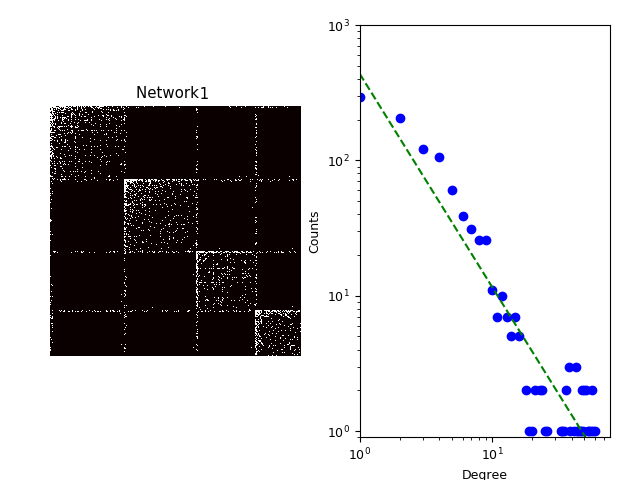
\includegraphics[width=1.1\textwidth]{img/corpus/network1_dd}
        \end{minipage}
        \begin{minipage}{0.24\textwidth}
            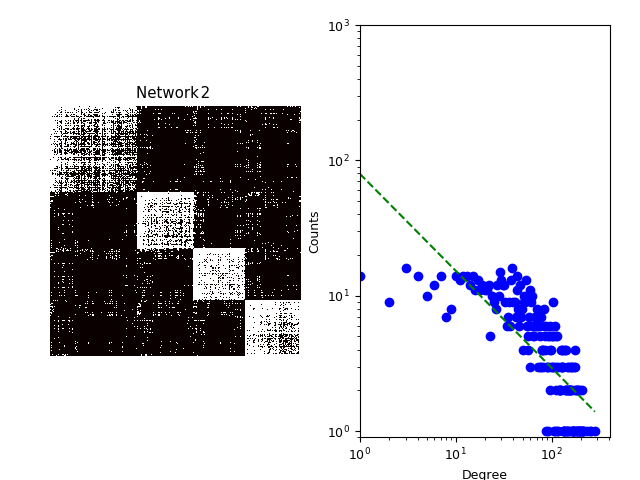
\includegraphics[width=1.1\textwidth]{img/corpus/network2_dd}
        \end{minipage}
        %\vskip\baselineskip
        \begin{minipage}{0.24\textwidth}
            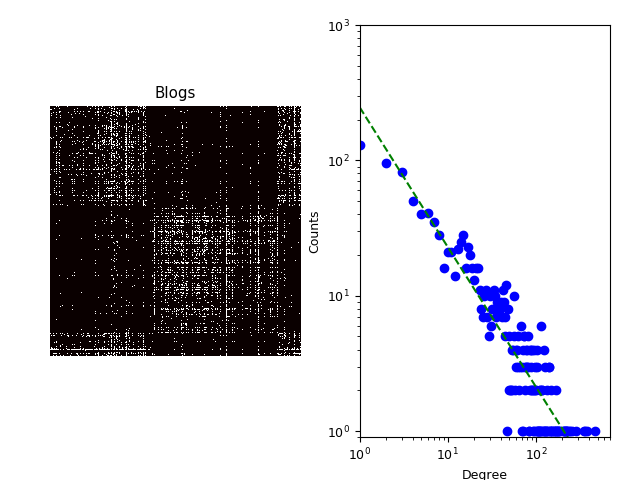
\includegraphics[width=1.1\textwidth]{img/corpus/blogs_dd}
        \end{minipage}
        \begin{minipage}{0.24\textwidth}
            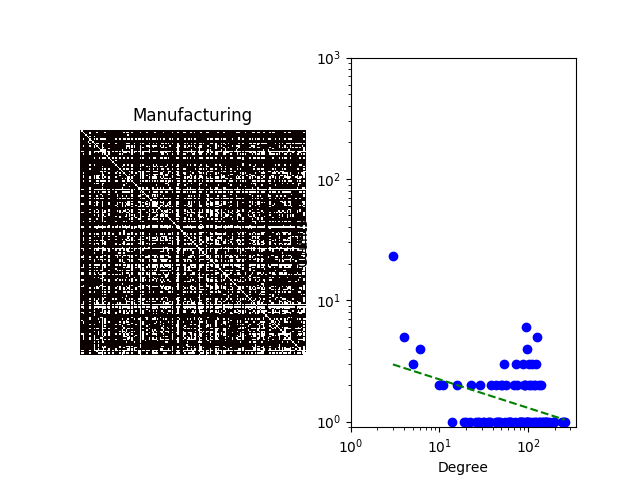
\includegraphics[width=1.1\textwidth]{img/corpus/manufacturing_dd}
        \end{minipage}
	\caption{Adjacency matrices (left) and global degree distributions (right) for the four training datasets. In the adjacency matrices, a white dot corresponds to a 1 and a block dot to a 0.}
	\label{fig:corpuses}
\end{figure}

\begin{figure}[h]
        \begin{minipage}{0.24\textwidth}
            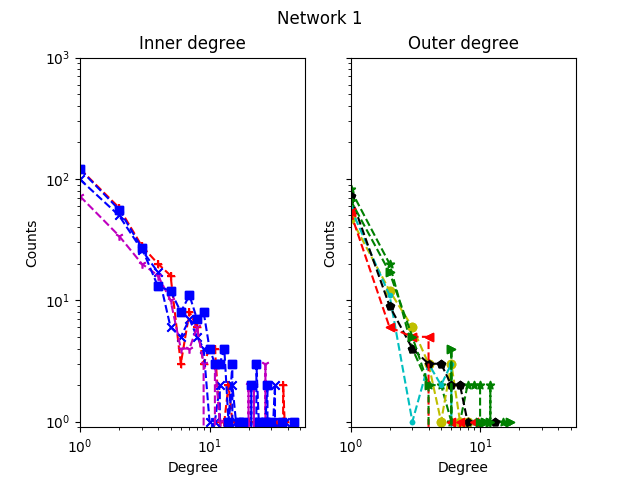
\includegraphics[width=4.22cm,height=3.5cm]{img/corpus/network1_1}
        \end{minipage}
        \begin{minipage}{0.24\textwidth}
            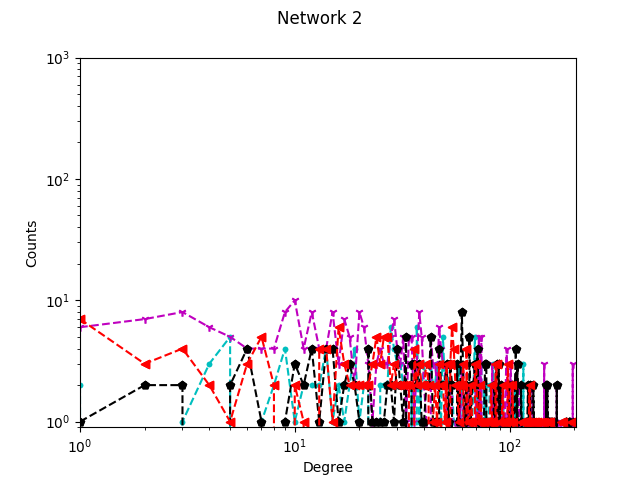
\includegraphics[width=4.22cm,height=3.5cm]{img/corpus/network2_1}
        \end{minipage}
        \vskip\baselineskip
        \begin{minipage}{0.24\textwidth}
            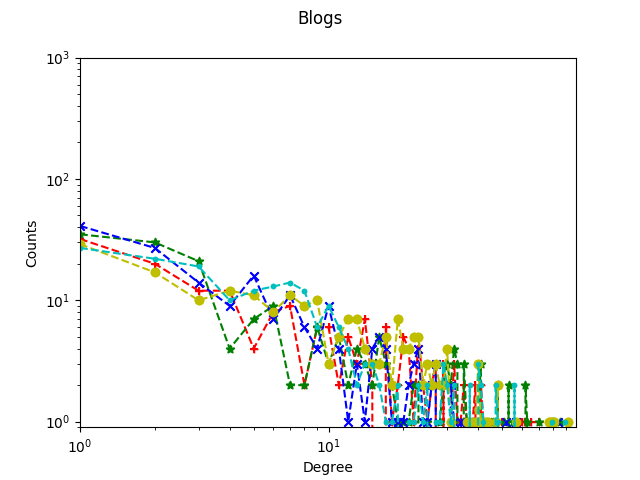
\includegraphics[width=4.22cm,height=3.5cm]{img/corpus/blogs_1}
        \end{minipage}
        \begin{minipage}{0.24\textwidth}
            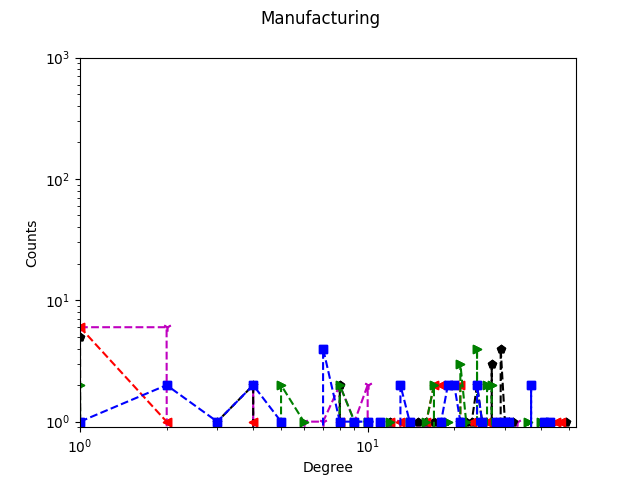
\includegraphics[width=4.22cm,height=3.5cm]{img/corpus/manufacturing_1}
        \end{minipage}
        \caption {Local degree distributions for the four training datasets. For Network1 and Network2 the classes come from ground-truth. For Blogs and Manufacturing, classes are obtained by the Louvain algorithm.} 
	\label{fig:synt_graph_local}
\end{figure}

For each dataset, we estimate the model parameters through Markov Chain Monte Carlo inference consisting of 200 iterations. For \imb, the concentration parameters of HDP were optimized  using vague gamma priors $\alpha_0 \sim \text{Gamma}(1,1)$ and $\gamma \sim \text{Gamma}(1,1)$ following \cite{HDP}. The parameters for the matrix weights  $\lambda_0$ and $\lambda_1$ were fixed to 0.1. For \ifm, the hyperparameter  $\sigma_w$ was fixed to 1 and the IBP hyperparameter $\alpha$ to 0.5 in order to  have comparable number of classes with \imb. Once the models have been learned, they are used to generate links (or non-links) between the entire set of network nodes. The whole procedure is repeated 10 times and the average values are reported as final results.

\subsection{Homophily}

Figure \ref{fig:homo_mustach} presents boxplots describing the distributions of the natural $s_n(i,j)$ and latent $s_l(i,j)$ similarities computed respectively on linked and non-linked pairs of nodes for \imb\ (left) and \ifm\ (right). The results have been aggregated over the four datasets. They confirm that the natural similarity is  higher for pairs of nodes which are linked than for pairs of nodes which are not linked, for both models. For the latent similarity,  there is no difference between the linked and non-linked pairs, indicating that the links are not homophilic. These experimental results are in line with the theoretical results presented in Section~\ref{sec:homophily} that state that both \ifm\ and \imb\ are homophilic with respect to the natural similarity but are not homophilic for the latent similarity.

\begin{figure}[ht]
\centering
    \begin{subfigure}
       	 \centering
        	 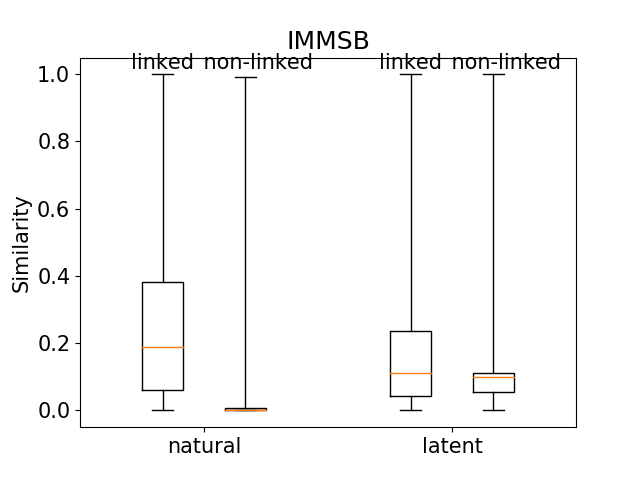
\includegraphics[width=4.22cm,height=3.5cm]{img/corpus/homo_mustach_immsb}
    \end{subfigure}
    \begin{subfigure}
        	 \centering
          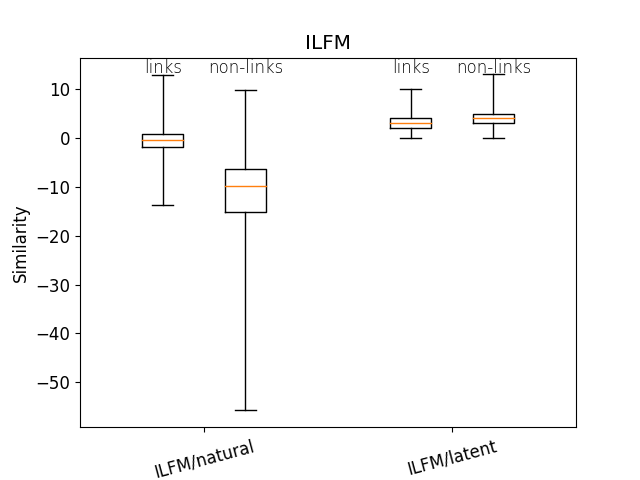
\includegraphics[width=4.22cm,height=3.5cm]{img/corpus/homo_mustach_ilfm}
    \end{subfigure}
    \caption{Natural and latent similarities aggregated over all datasets and computed on linked and non-linked pairs of nodes for \imb\ (left) and \ifm\ (right).}
    \label{fig:homo_mustach}
\end{figure}

\subsection{Preferential attachment}

Table \ref{table:me_gofit} reports the value of the power-law goodness of fit for \imb\ and \ifm\ in the global case (left) and in the local case (right). It appears that for both models, the global preferential attachment is only verified for networks generated from datasets where the property was observed, namely in Network1 with p-value equals to 0.9 for \imb\ and 1 for \ifm, and in Blogs with a p-value equals to 1 for the both models; the property is not verified in Network2 and in Manufacturing, where p-values equal 0. This is in accordance with Proposition 2.1 according to which both \ifm\ and \imb\ do not satisfy global preferential attachment. However, these models are able to capture this property if it exists in the training datasets.  Moreover, one can observe that, in the local case, \imb\ complies with the preferential attachment with $p$-values equals or close to 1 for the four networks, while \ifm\ obtained low p-values for the networks that were less locally bursty (respectively equal to 0 and 0.3 for Network2 and Manufacturing). In addition, the power-law coefficients $\alpha$ are significantly greater for \imb\ than for \ifm, and specially for the bursty networks Network1 and Blogs.

Figure \ref{fig:me_local} illustrates the local preferential attachment for Network1 (top) and Network2 (bottom) estimated with \imb\ (left) and \ifm\ (right). The shape of local degree distributions appears more linear for \imb\ and with more fluctuations for \ifm. This illustrates the fact that \ifm\ does not capture local preferential attachment whereas \imb\ does, as stated in Proposition 2.2. 


\begin{table}[h]{Preferential attachment measures for training datasets and networks generated with fitted models.}
\begin{tabular}{lrrrr}
  \multirow{2}{*}{\textbf{Training Datasets}}  &
  \multicolumn{2}{c}{Global} & \multicolumn{2}{c}{Local}\\
  \cmidrule(r){2-3} \cmidrule(l){4-5}
  &   $p$-value &   $\alpha$   & $p$-value & $\alpha$   \\
\hline
Network1       & 1 & 2.4 &   1.0 $\pm$ 0.0  &  1.8 $\pm$ 0.03  \\
Network2       & 0 & 1.3 &   0.0 $\pm$ 0.0  &  1.2 $\pm$ 0.01 \\
Blogs          & 1 & 1.5 &   1.0 $\pm$ 0.0  &  1.4 $\pm$ 0.03\\
Manufacturing  & 0 & 1.4 &   0.4 $\pm$ 0.3  &  1.3 $\pm$ 0.05 \\
\hline

  \ \textbf{\immsb} &&&& \\
\hline
Network1       & 0.9 & 1.4 &   1.0 \(\pm\) 0.0   &  3.5 \(\pm\) 0.7 \\
Network2       & 0 & 1.3 &   0.9 \(\pm\) 0.0   &  1.6 \(\pm\) 0.2 \\
Blogs          & 1 & 1.3 &   1.0 \(\pm\) 0.0   &  4.3 \(\pm\) 1.1 \\
Manufacturing  & 0 & 1.2 &   0.9 \(\pm\) 0.01  &  1.6 \(\pm\) 0.1 \\
\hline

  \ \textbf{\ilfm} &&&& \\
\hline
Network1      & 1 & 1.4 &   1.0 \(\pm\) 0.0  &  1.7 \(\pm\) 0.1 \\
Network2      & 0 & 1.2 &   0.0 \(\pm\) 0.0 &  1.2 \(\pm\) 0.0 \\
Blogs         & 1 & 1.3 &   0.9 \(\pm\) 0.2  &  1.5 \(\pm\) 0.1 \\
Manufacturing & 0 & 1.2 &   0.3 \(\pm\) 0.3  &  1.3 \(\pm\) 0.0 \\
\hline
\end{tabular}
\label{table:me_gofit}
\end{table}

\begin{figure}[h]
    \begin{minipage}{0.24\textwidth}
        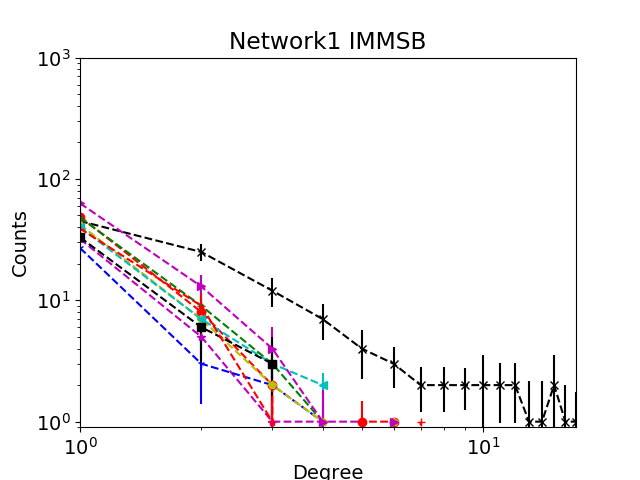
\includegraphics[width=4.22cm,height=3.5cm]{img/corpus/immsb_network1_1}
    \end{minipage}
    \begin{minipage}{0.24\textwidth}
        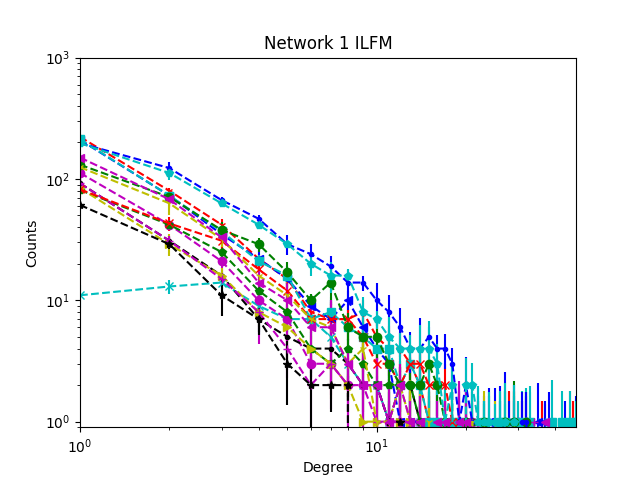
\includegraphics[width=4.22cm,height=3.5cm]{img/corpus/ilfm_network1_1}
    \end{minipage}
    \vskip\baselineskip
    \begin{minipage}{0.24\textwidth}
        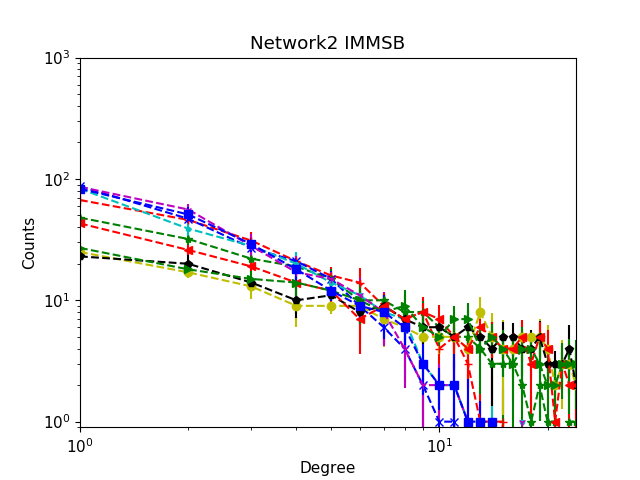
\includegraphics[width=4.22cm,height=3.5cm]{img/corpus/immsb_network2_1}
    \end{minipage}
    \begin{minipage}{0.24\textwidth}
        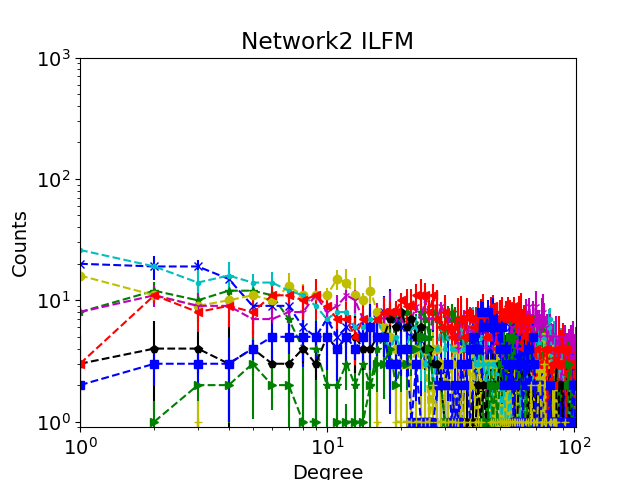
\includegraphics[width=4.22cm,height=3.5cm]{img/corpus/ilfm_network2_1}
    \end{minipage}
    \caption {Local degree distributions for Network1 (top row) and Network2 (bottom row) generated with fitted models \imb\ (first column) and \ifm\ (second column).} 
\label{fig:me_local}
\end{figure}

\begin{figure}[h]
\centering
    \begin{minipage}{0.24\textwidth}
        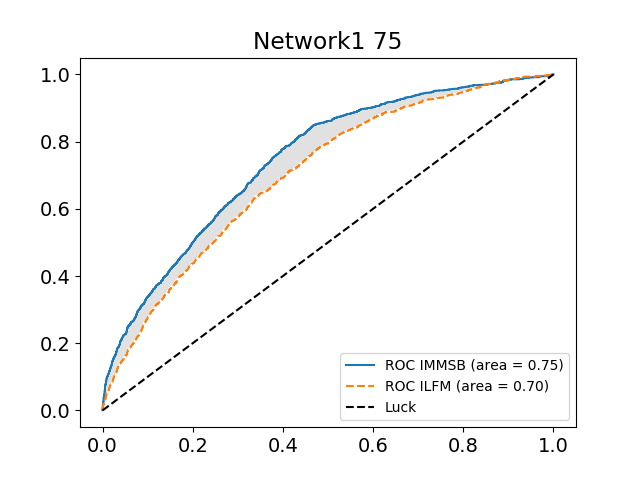
\includegraphics[width=4.22cm,height=3.5cm]{img/corpus/roc_network1_75_f}
    \end{minipage}
    \begin{minipage}{0.24\textwidth}
        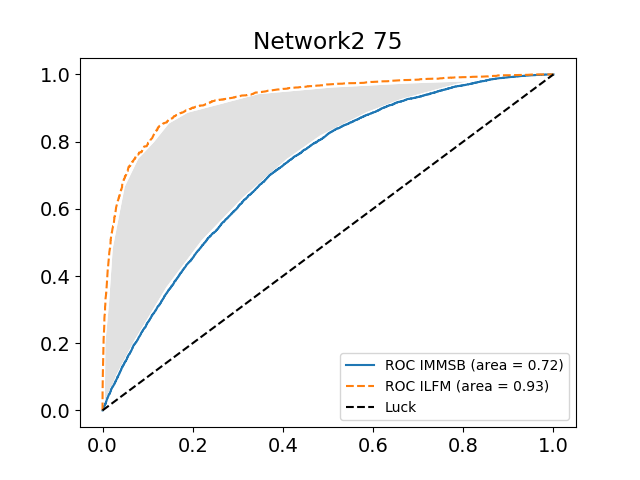
\includegraphics[width=4.22cm,height=3.5cm]{img/corpus/roc_network2_75_f}
    \end{minipage}
    \begin{minipage}{0.4\textwidth}
        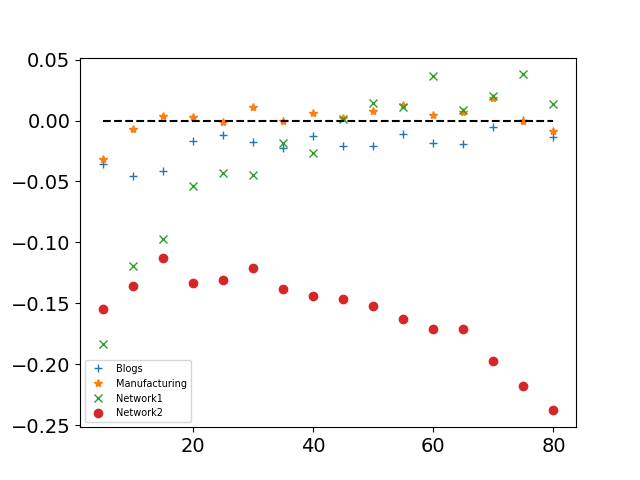
\includegraphics[width=\textwidth]{img/corpus/testset_max_20.png}
    \end{minipage}
    \caption{Top: AUC-ROC curves for Network1 (left) and Network2 (right) with 20 percent of data used as learning set. Bottom: Relative performance of \imb\ and \ifm\ acc. to the percentage of data used as testing set (the remainder being used for learning).} 
\label{fig:auc}
\end{figure}

Lastly, Figure \ref{fig:auc} compares the performance of the models for predicting new links using the Area Under the Curve (AUC) measure as a function of the training set size. In the bottom plot, the y-axis gives the relative performance defined as the difference of the AUC values for \imb\ and \ifm\ ($AUC_{\imb} - AUC_{\ifm}$) whereas the x-axis indicates the percentage of links randomly removed from the datasets and used as testing set. Hence, the number of training data decreases with the x-axis and a positive value on the y-axis indicates that \imb\ outperforms \ifm.  Note that the relative performance corresponds to the difference of the MAX AUC values obtained for both models on the ten inference experiences. The top plot illustrates a case where 20 percent of the data is used as testing set and where \imb\ dominates \ifm\ on Network1 (left) and the opposite for Network2 (right).

In general, as shown in the bottom plot, \ifm\ obtains better performance than \imb. However, the relative predictive performance of \imb\  increases  when the quantity of training data decreases on bursty networks, whereas for non-bursty networks the results are the opposite: the performance of \ifm\ increases when the size of the learning dataset decreases. This is particularly visible for Network2; this is less visible on Manufacturing, certainly due to the small size of this network, which makes the prediction less challenging.

The above behavior can be explained by the fact that \imb\ satisfies the local preferential attachment whereas \ifm\ does not: as links are randomly removed, one is more likely to remove links from large classes than from small ones; a model that enforces local preferential attachment on bursty networks is thus more likely to reconstruct those removed links. This is what is happening on Network1 and Blogs for \imb. On the contrary, for non-bursty networks, a model enforcing local preferential attachment is penalized.

\section{Conclusion}

We have studied here whether stochastic mixed membership models, such as \ifm\ and \imb\, can generate new links while satisfying properties frequently verified in real  social networks, namely homophily and preferential attachment. To do so, we have introduced formal definitions of these properties and have analyzed how these models behave according to those definitions. We have shown, in particular, that both models are \textit{homophilic} with the natural similarity that underlies them. Concerning preferential attachment, we have shown that stochastic mixed membership models do not comply with global preferential attachment. The situation is however more contrasted when the property is considered at the local level: \imb\ enforces local preferential attachement whereas \ifm\ does not.

These findings have been validated experimentally on two real and two artificial networks that have different degrees of global and local preferential attachment. An important, practical finding of our study is that \imb, usually considered of lesser "quality" than \ifm, can indeed yield better results on bursty networks (\textit{i.e.} networks with preferential attachment) when the number of training data is limited.
% This study also paves the way to new models enforcing global preferential attachment through a strict adherence to the definition we have provided.

\bibliographystyle{unsrt}
\bibliography{./pnas}

\end{document}
